\documentclass[journal]{IEEEtran}
\usepackage{booktabs} \usepackage{array} \usepackage{tabularx}
\usepackage{epsfig,rotating,setspace,latexsym,amsmath,epsf,amssymb,amsfonts,bm,theorem,cite,caption,subcaption,enumerate,longtable,accents}
\usepackage{algorithm,algorithmic,graphicx,epsf,authblk,epstopdf,url,color,multirow,lettrine}
\usepackage{tabularx}



\newtheorem{theorem}{Theorem}
\newtheorem{problem}{Problem}
\newtheorem{corollary}{Corollary}
\newtheorem{definition}{Definition}
\newtheorem{remark}{Remark}
\newtheorem{lemma}{Lemma}
\newenvironment{Proof}[1]{\medskip\par\noindent{\bf Proof:\,}\,#1}{{\mbox{\,$\blacksquare$}\par}}

\allowdisplaybreaks

\begin{document}

\title{Special-Purpose Motors: An Overview}
\author{Ahmed Aly, Ahmed Sherif Ahmed
, Kerollos Saad Thomas, Yahia Eldakhakhny, and Youssef El-Sayed}


\maketitle

\begin{abstract}	
Machines are everywhere. Some types were invented to serve a special purpose. These special-purpose motors excelled in many ways over their counterparts. That makes studying them necessary and important. The motors in discussion have a lot of important daily life applications. As such, these motors will be covered in good detail in this report. The aim is to summarize the theory and discuss the applications thoroughly. 
\end{abstract}


\begin{IEEEkeywords}
    Electric Machinery, Special-Purpose Motors, Induction Motor, Universal Motor, Stepper Motor, Hybrid Stepper Motor.    	
\end{IEEEkeywords}


\section{Introduction}	

Since the discovery of electricity till our day, electrical machines have been a crucial part of our lives; from domestic use in blenders, refrigerators and washing machines to the industrial use in production lines. This evolution was lead by the invention of special purpose machines; whose working principle
%%Kero:
is based on the conventional old motors but enhanced to serve special purposes. Surpassing even the efficiency of the old motors in theses special fields of use.

In this report, the topic of special purpose electrical machines is covered, with more interest in three machines: Universal Motor, Single Phase Induction Motor, and Stepper Motor.
Supported with illustrations and equations, this report covers the main theory of operation, types, applications, advantages and disadvantages of each of the machines mentioned before.



\section{Single-Phase Induction Motor}

\begin{figure}[h]
    \centering
    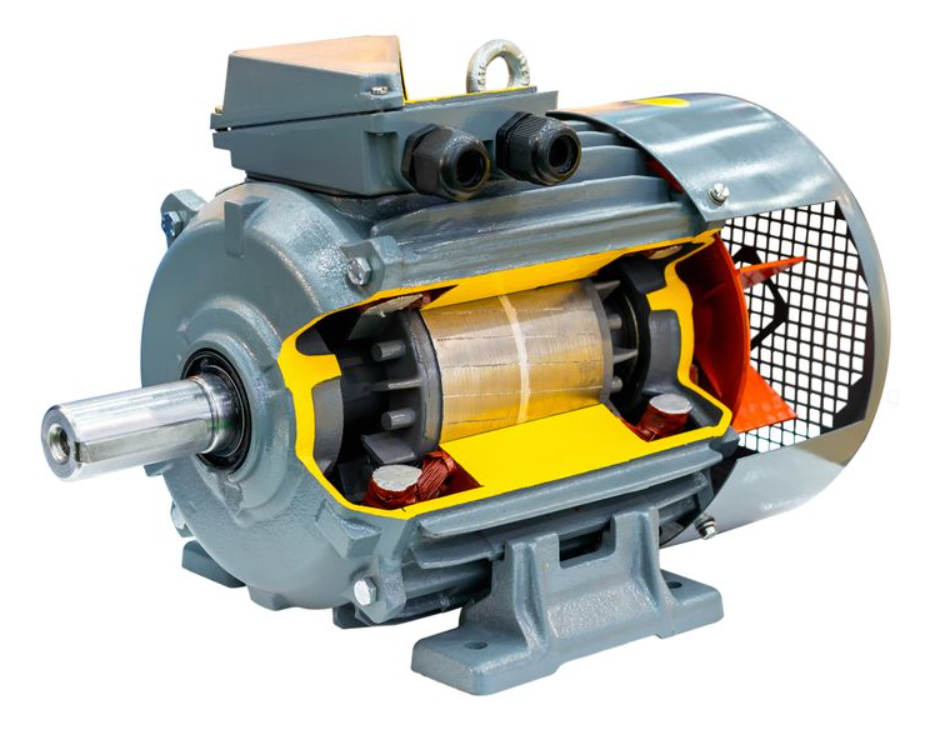
\includegraphics[scale=0.27]{Induction/single-phase-induction-motor.PNG}
    \caption{Single-Phase Motor \cite{single_phase_ind}}
\end{figure}
Single-Phase induction motors are singly-fed motors. They operate on the premise of induction; where the magnetic field generated at the stator is used to power-up and drive the rotor, allowing it to rotate and supply mechanical power. It is a general consensus that this motor is, by and large, a transformer with a rotating secondary winding.
%%%%%%%%%%%%%%%%%
\subsection{Theory of Operation}
This section will briefly discuss the theory of operation of three-phase induction motors; then dive deep into that of single-phase in detail.
\subsubsection{Three-Phase Induction Motor (TPIM)}
Operation can be summarized as follows:
\begin{itemize}
    \item When the stator windings are excited by a three-phase power supply, a rotating magnetic field is generated; whose speed is denoted as $N_s$ \cite{tamer}\cite{guru2007}, and given by equation \ref{threephase_ns}; where $f_s$ represents the supply frequency, and $P$ represents the number of poles.
    \begin{equation}
        N_s = 120\frac{f_s}{P}
        \label{threephase_ns}
    \end{equation}
    
    \item The generated magnetic field cuts the rotor's windings; inducing an electromotive force in it, and a current is produced upon short circuiting its terminal \cite{tamer}\cite{guru2007}.
    
    \item This flowing current causes the rotor to rotate by a speed $N_r$ in the same direction with $N_s$. So, the relative speed —also known as slip speed— between stator field and rotor\cite{tamer} becomes as shown in equation \ref{threephase_rel}. The slip speed is more often than not expressed by the slip $s$ \cite{guru2007}; which is given as shown in equation \ref{threephase_slip}. 
    \begin{equation}
        (N_s - N_r)
        \label{threephase_rel}
    \end{equation}
    \begin{equation}
        s = \frac{N_r - N_s}{N_r}
        \label{threephase_slip}
    \end{equation}
    \item The starting torque is primarily controlled by the rotor's effective resistance; which is dependant on the per-unit-slip $s$.
    \begin{equation}
        T_{st} \propto R_2
    \end{equation}
    
\end{itemize}

\subsubsection{Single-Phase Induction Motor (SPIM)}
Suppose that a single-phase voltage supply —that increases in the upward direction— is feeding the stator of an SPIM; causing current flow. This current —according to Faraday's law— produces a \textbf{pulsating} magnetic field in each winding that also increases in the upward direction. The generated magnetic field causes a flow of current —in a direction opposite to the field causing it— in the rotor's two conductors. As shown in figure \ref{fig:rotorsingle}, each of the current-carrying conductors experience a force that wants to rotate the rotor; each in a direction opposite to the other; rendering it in a state of rest. Thus; resulting in a starting torque of zero.
\begin{figure}[h]
    \centering
    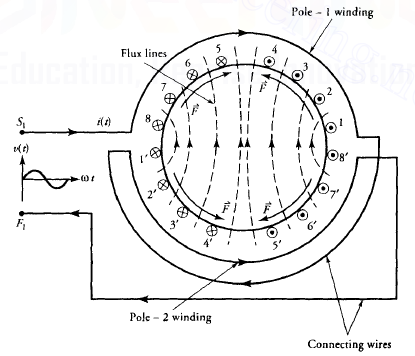
\includegraphics[scale=0.5]{Induction/single_construction.PNG}
    \caption{Current-Carrying Conductors in Rotor \cite{guru2007}}
    \label{fig:rotorsingle}
\end{figure}
\newline
This phenomenon is explained by \textit{Double Revolving-Field Theory}; which states that a pulsating magnetic field can be resolved into two revolving magnetic fields equal in magnitude and opposite in direction —one rotating clockwise and the other anticlockwise \cite{guru2007}.
\begin{figure}[h]
    \centering
    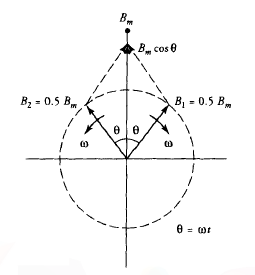
\includegraphics[scale=0.50]{Induction/double_revolving.PNG}
    \caption{Resolving a Pulsating Field into Two Rotating Fields \cite{guru2007}}
    \label{fig:rotorsingle}
\end{figure}
\newline
Let the section of the rotor circuit getting affected by the clockwise-field be called the \textbf{forward branch} and the one getting affected by the anticlockwise-field be called the \textbf{backward branch}. At standstill, the impedance and the current in both forward and backward branches are equal; also the torques affecting both are equal in magnitude but opposite in direction. If the rotor was able to rotate clockwise at a speed $N_r$, knowing that the speed of the clockwise field is $N_s$ and, similarly, the speed of the anticlockwise field is $-N_s$; the slip can be formulated by equations \ref{equsf} and \ref{equsb}, where $s_f$ is the forward slip and $s_b$ is the backward slip.
\begin{equation}
    s_f = \frac{N_s -  N_r}{N_s} = 1- \frac{N_r}{N_s}
    \label{equsf}
\end{equation}
\begin{equation}
    s_b = \frac{-N_s - N_r}{-N_s} = 1 + \frac{N_m}{N_s} = 2 - s
    \label{equsb}
\end{equation}
In order for the motor to rotate, the value of $s$ has to be less than 1; that causes the effective resistance in the forward branch to be greater than that of the backward branch; developing a resultant torque in the forward direction as a result \cite{guru2007}. This will only be able to be achieved, however; by either applying an external torque in any direction, or by starting the motor using external circuitry to circumvent this problem.
\newline

%%%%%%%
\subsection{Three-Phase and Single-Phase Induction Motors: A Comparison}
This section aims to dissect the differences between TPIM and SPIM; going through each point in detail.
\subsubsection{Construction}
\begin{itemize}
    \item \textbf{Three-Phase induction motor} consists of a stator similar in construction to synchronous machines, and either a wound rotor or a squirrel-cage rotor; depending on the type of application it is used in\cite{tamer}. This is shown in figure \ref{fig:threecons}.
    \begin{figure}[h]
    \centering
    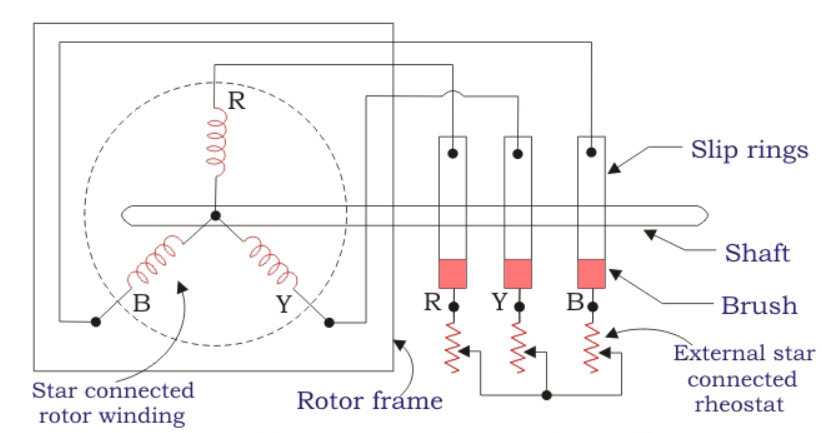
\includegraphics[scale=0.35]{Induction/three_construction.PNG}
    \caption{Construction of Three-Phase Motor \cite{three_construction}}
    \label{fig:threecons}
    \end{figure}
    
    \item \textbf{Single-Phase induction motor's} main distinction when it comes to construction is the fact that its stator contains two windings; main and auxiliary. This is shown in figure \ref{fig:singlecons}.
    \begin{figure}[h]
    \centering
    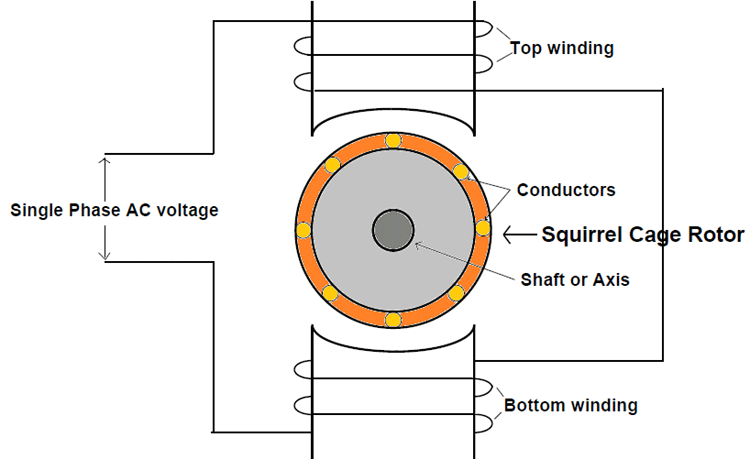
\includegraphics[scale=0.27]{Induction/Single-Phase-Induction-Motor (1).png}
    \caption{Construction of Single-Phase Motor \cite{single_construction}}
    \label{fig:singlecons}
    \end{figure}
\end{itemize}

%%%%%%%%%%

\subsubsection{Operating Conditions}
\begin{itemize}
    \item \textbf{Three-Phase induction motor} operates when the starting torque is more than the load torque; so, the magnetic force applied on the rotor will case it to rotate in the same direction as the rotating field \cite{tamer}\cite{guru2007}. 
    
    \item \textbf{Single-phase induction motor} operates when the starting torque is more than the load torque and the motor is made to rotate by an external torque —or with the help of external circuitry; so that the torque developed in the forward branch is higher than the torque in the backward branch.\cite{guru2007}.
    
    
\end{itemize}




\subsubsection{Type of Field}
\begin{itemize}
    \item The type of field generated in \textbf{three-phase induction motors} is a rotating magnetic field\cite{tamer}.
    \item The type of field generated in \textbf{single-phase induction motors} is a pulsating magnetic field.
\end{itemize}
\subsubsection{Self-Starting}
\begin{itemize}
    \item \textbf{Three-Phase induction motors} are inherently self-starting.
    \item \textbf{Single-Phase induction motors} require modifications to self-start.
\end{itemize}


\subsubsection{Per-Unit Slip Formula}
\begin{itemize}
    \item The per-unit-slip formula\cite{tamer} for \textbf{three-phase induction motor} is given by
    \begin{equation}
        s = 1 - \frac{N_s}{N_r}
    \end{equation}
    
    \item The per-unit-slip for \cite{guru2007} \textbf{single-phase induction motor} has 2 formulas; because the generated magnetic field has 2 components rotating in opposite directions. So, it is given by 
    \begin{equation}
        s = 1 - \frac{N_s}{N_r}
    \end{equation} 
    \begin{equation}
        s_b = 1 + \frac{N_s}{N_r} = 2 - s
    \end{equation}
\end{itemize}



\subsubsection{Equivalent Circuit}
\begin{itemize}
    \item The equivalent circuit for \textbf{three-phase induction motor} is shown in figure \ref{fig:threecir}.
    \begin{figure}[h]
    \centering
    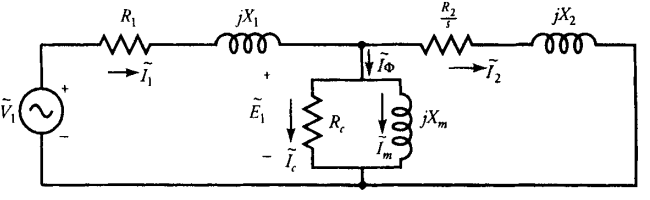
\includegraphics[scale=0.40]{Induction/three_circuit.PNG}
    \caption{Circuit Schematic for Three-Phase Motor \cite{guru2007}}
    \label{fig:threecir}
    \end{figure}
    
    \item The equivalent circuit for \textbf{single-phase induction motor} is shown in figure \ref{fig:singlecir}.
    \begin{figure}[h]
    \centering
    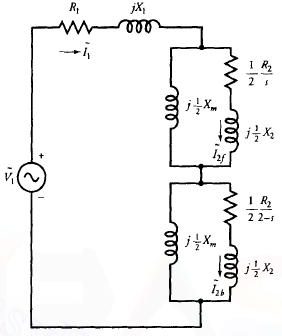
\includegraphics[scale=0.55]{Induction/single_circuit.PNG}
    \caption{Circuit Schematic for Single-Phase Motor \cite{guru2007}}
    \label{fig:singlecir}
    \end{figure}
\end{itemize}



\subsubsection{Speed-Torque Characteristics}
\begin{itemize}
    \item The speed-torque characteristics graph for \textbf{three-phase induction motor} is shown in figure \ref{fig:threetor}.
    \begin{figure}[h]
    \centering
    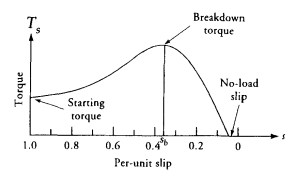
\includegraphics[scale=0.6]{Induction/three_torque.PNG}
    \caption{Speed-Torque Characteristics for Single-Phase Motor \cite{guru2007}}
    \label{fig:threetor}
    \end{figure}
    
    \item The speed-torque characteristics graph for \textbf{three-phase induction motor} is shown in figure \ref{fig:singletor}.
    \begin{figure}[h]
    \centering
    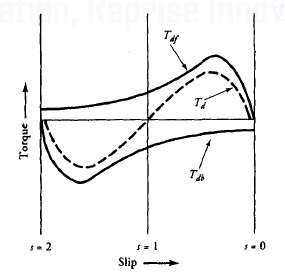
\includegraphics[scale=0.55]{Induction/single_torque.PNG}
    \caption{Speed-Torque Characteristics for Single-Phase Motor \cite{guru2007}}
    \label{fig:singletor}
    \end{figure}
    
\end{itemize}



\subsubsection{Types}
\begin{itemize}
    \item \textbf{Three-Phase induction motor} has two types depending on the type of rotor used: Squirrel-Cage, and Wound-Rotor\cite{tamer}.
    \item \textbf{Single-Phase induction motor} has four types: Split-Phase, Capacitor-Start, Capacitor-Start Capacitor-Run, and Permanent Split Capacitor.
\end{itemize}

% \begin{table}[]
% \begin{tabular}{@{}cll@{}}
% \toprule
% POC & \multicolumn{1}{c}{Single-Phase Induction Motor} & Three-Phase Induction Motor \\ \midrule
% Construction                 &                                                  &                             \\
% Operating Conditions         &                                                  &                             \\
% Self-Starting                &                                                  &                             \\
% Per-Unit Slip                &                                                  &                             \\
% Type of Field                &                                                  &                             \\
% Equivalent Circuit           &                                                  &                             \\
% Speed-Torque Characteristics &                                                  &                             \\
% Types                        &                                                  &                             \\ \bottomrule
% \end{tabular}
% \end{table}















%%%%%%%%
\subsection{Types of Single-Phase Induction Machines}
\subsubsection{Split-Phase Motor}
This motor is mostly used in mechanical applications that require fractional horsepower range. It contains two windings that are placed in space quadrature and connected in parallel to a single-phase source: main winding; which has low resistance and high inductance, and auxiliary winding; which has high resistance and low inductance. This motor's distinguishing feature is that the two windings carry out-of-phase currents. In fact, the phase difference between the two currents may reach 60\textdegree. The presence of auxiliary winding is mainly to provide high starting-torque —ranging between 150\% to 200\% of the full-load torque— and a high starting current. This winding is then separated when the motor attains 75\% of its speed to prevent excessive power loss\cite{guru2007}. Figures \ref{fig:splitphasesch} and \ref{fig:splitphasegraph} respectively showcase a schematic representation for this motor and its speed-torque graph.
\begin{figure}[h]
    \centering
    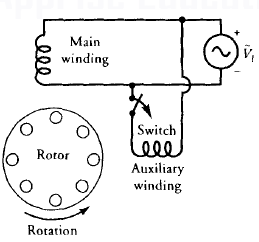
\includegraphics[scale=0.60]{Induction/split_phase_sch.PNG}
    \caption{Schematic Representation of Split-Phase Motor \cite{guru2007}}
    \label{fig:splitphasesch}
\end{figure}
\begin{figure}[h]
    \centering
    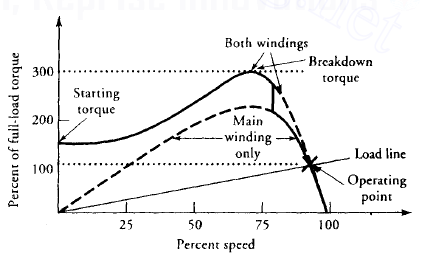
\includegraphics[scale=0.55]{Induction/split_phase_graph.PNG}
    \caption{Speed-Torque Graph of Split-Phase Motor \cite{guru2007}}
    \label{fig:splitphasegraph}
\end{figure}
%%%%%%%%%%%%%%%%End of Split-Phase%%%%%%%%%%%%%%%%%%%%%%%
\subsubsection{Capacitor-Start Motor}
In this motor, a capacitor —of carefully chosen value— is connected in series with auxiliary winding; this is done to make the auxiliary-winding current lead the main-winding current by exactly 90\textdegree. This results in a starting torque that is as good as that of three-phase motors. Similar to split-phase motor; the auxiliary winding is disconnected when the motor reaches 75\% of its speed by a centrifugal switch, along with the series capacitor. Capacitor-Start motor is primarily used in applications that require a starting torque that is 4 to 5 times the rated torque\cite{guru2007}. Figures \ref{fig:capstartsch} and \ref{fig:capstartsgraph} respectively showcase a schematic representation for this motor and its speed-torque graph.
\begin{figure}[h]
    \centering
    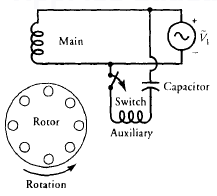
\includegraphics[scale=0.67]{Induction/cap_start_sch.PNG}
    \caption{Schematic Representation of Capacitor-Start Motor \cite{guru2007}}
    \label{fig:capstartsch}
\end{figure}
\begin{figure}[h]
    \centering
    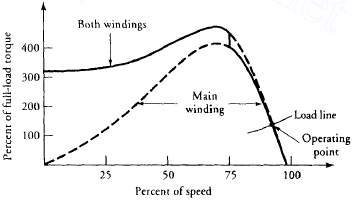
\includegraphics[scale=0.57]{Induction/cap_start_graph.PNG}
    \caption{Speed-Torque Graph of Capacitor-Start Motor \cite{guru2007}}
    \label{fig:capstartsgraph}
\end{figure}
%%%%%%%%%%%%%%%%End of Cap-Start%%%%%%%%%%%%%%%%%%%%%%%
\subsubsection{Capacitor-Start Capacitor-Run Motor}
This motor fixes one of the biggest drawbacks split-phase and capacitor-start motors; the low power factor when running at rated speed, leading to an efficiency as low as 50\% to 60\%. This motor improves the power factor by employing a second capacitor —the first is used to improve starting torque— when it runs at rated speed; thus, elevating the power factor and improving the efficiency\cite{guru2007}. Figures \ref{fig:capstcaprunsch} and \ref{fig:capstcaprungraph} respectively showcase a schematic representation for this motor and its speed-torque graph.

\begin{figure}[h]
    \centering
    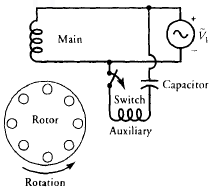
\includegraphics[scale=0.67]{Induction/cap_start_cap_run_sch.PNG}
    \caption{Schematic Representation of Capacitor-Start Capacitor-Run Motor \cite{guru2007}}
    \label{fig:capstcaprunsch}
\end{figure}
\begin{figure}[h]
    \centering
    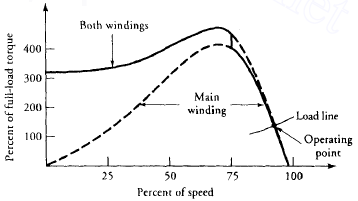
\includegraphics[scale=0.57]{Induction/cap_start_cap_run_graph.PNG}
    \caption{Speed-Torque Graph of Capacitor-Start Capacitor-Run Motor \cite{guru2007}}
    \label{fig:capstcaprungraph}
\end{figure}
%%%%%%%%%%%%%%%%End of Cap-Start Cap-Run%%%%%%%%%%%%%%%%%%%%%%%
\subsubsection{Permanent Split Capacitor Motor}
This motor is a more cost-effective version of capacitor-start capacitor-run (CSCR) motor; where it only employs one capacitor for both starting and performance enhancement. Therefore, its starting torque is relatively low when compared to CSCR motor. But, it is more suitable for applications that require frequent starting and does not need a high starting torque. It also comes in a size smaller than any of the motors mentioned above; due to the elimination of the centrifugal switch —since it does not disconnect the capacitor when it reaches 75\% of its speed\cite{guru2007}.

Figures \ref{fig:permsplitcapsch} and \ref{fig:permsplitcapgraph} respectively showcase a schematic representation for this motor and its speed-torque graph.

\begin{figure}[h]
    \centering
    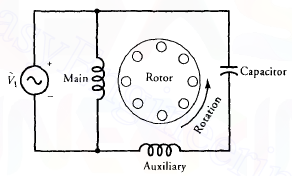
\includegraphics[scale=0.60]{Induction/perm_split_cap_sch.PNG}
    \caption{Schematic Representation of Permanent Split Capacitor Motor \cite{guru2007}}
    \label{fig:permsplitcapsch}
\end{figure}
\begin{figure}[!h]
    \centering
    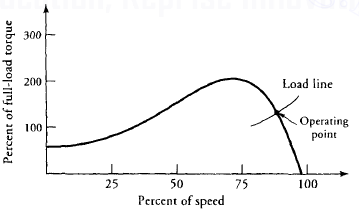
\includegraphics[scale=0.57]{Induction/perm_split_cap_graph.PNG}
    \caption{Speed-Torque Graph of Permanent Split Capacitor Motor \cite{guru2007}}
    \label{fig:permsplitcapgraph}
\end{figure}

%%%%%%%%%%%%%%%%%%%%%%%End of Types%%%%%%%%%%%%%%%%%%%%%%
%%%%%%%%%%%%%%%%%%%%%%%%%%%%%%%%%%%%%%%%%%%%%%%%%%%%%%%%%
\subsection{Advantages and Disadvantages of Single-Phase Induction Motor}
\subsubsection{Advantages}
\begin{itemize}
    \item SPIM lightweight and compact.
    \item SPIM has a relatively high efficiency.
    \item SPIM does not require constant maintenance and has a long lifetime\cite{adv_induction1}.
    \item SPIM can be designed in a variety of sizes to fit many applications\cite{adv_induction1}.
\end{itemize}
\subsubsection{Disadvantages}
\begin{itemize}
    \item SPIM is not inherently self-starting\cite{adv_induction1}.
    \item SPIM has lower power factor and efficiency when compared with its three-phase counterpart\cite{adv_induction1}. 
\end{itemize}

%%%%%%%%%%%%%%%%%%%%End of Adv and Dis%%%%%%%%%%%%%%%%%%%%%%%%%
\subsection{Single-Phase Induction Motor Applications}
\begin{itemize}
    \item SPIMs are used in equipment and machinery that requires power ranging from a fraction of one horsepower to single-digit horsepower; like pumps, compressors, electric shavers, and drills\cite{uses_induction}.
    \item SPIMs are used for an electric drive for low-power constant speed machines when three-phase supply is not available\cite{uses_induction}.
\end{itemize}

% %%%%%%%%%%%%%End of Applications%%%%%%%%%%%%%%%

%%%%%%%%%%%%%%%%%%%%%%%%%%%%%%%%%%%%%%%%%%%%%%%%%%%%%%%%%%%%%%%%%%%%%%%%%%%%%%%%%%%%%%%%%%%%%%%%%%%%%%%%%%%%%%%%%%%%%%%%%%%%%%%%%%
%%%%%%%%%%%%%%%%%%%%%%%%%%%%%%%%%%%%%%%%%%%%End of Single-Phase Induction Motor%%%%%%%%%%%%%%%%%%%%%%%%%%%%%%%%%%%%%%%%%%%%%%%%%%%
%%%%%%%%%%%%%%%%%%%%%%%%%%%%%%%%%%%%%%%%%%%%%%%%%%%%%%%%%%%%%%%%%%%%%%%%%%%%%%%%%%%%%%%%%%%%%%%%%%%%%%%%%%%%%%%%%%%%%%%%%%%%%%%%%%

\section{Universal Motor}
\subsection{Introduction to Universal Motor}
When connecting an AC source to a DC series motor, where the armature and the field has the same current as in series motors, the generated torque is unidirectional as a result of reversing both the field flux and armature current, this is the basic idea of the universal motor. But AC sources produce undesirable behaviours when connected to normal DC motors, such as eddy currents and inductive reactance of the armature and the field.\cite{chapman2005}

\begin{figure}[h]
    \centering
    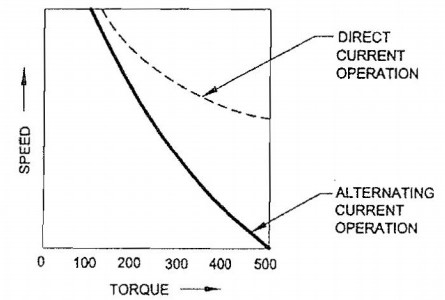
\includegraphics[scale=0.6]{universal/DC vs universal_google.jpg}
    \caption{DC vs AC operation of DC motor}
    \label{fig:DC vs uni}
\end{figure}

\subsection{Connecting a DC Motor to an AC Power Supply}
As shown in figure \ref{fig:DC vs uni}, the efficiency of a DC motor drops significantly once it is connected to an AC source and this is due to:
\begin{enumerate}
    \item AC produces Alternating flux, which increases the eddy currents, so a lot of energy is lost as heat causing the motor to be less efficient and heat more quickly.
    \item When the motor is connected with an AC supply, the effect of the inductive reactance of both the armature and field coils starts to impede the flow of current, so less current flows in the motor causing the motor to operate on a lower speed at the same input voltage, This newly introduced inductance lowers the total power factor of the motor.
    \item AC causes transformer action between the armature and field winding, which in turn produces induced emf, increasing the risk of sparks on the commutator, and shortening the lifetime of the brushes.\cite{guru2007}
\end{enumerate}


It is then evident that connecting a DC motor to an AC supply has serious drawbacks, but the effects of these drawbacks can be minimized by various means including:
\begin{enumerate}
    \item The effects of the eddy currents can be kept to a minimum by making the core and poles out of laminated layers.
    \item The number of commutator segments must be increased and the resistance of the brushes can be increased as well, so they can withstand sparks and friction.\cite{guru2007}
\end{enumerate}

\subsection{Main Differences Between Universal and DC Motors}
It is true that that the universal motor's core and poles are made of laminated layers, and its commutator has more segments, but those are not fundamental differences that differentiate it from any ordinary DC motor. The main difference between them is that the universal motor has an extra inductor connected in series with the armature winding as shown in figure  \ref{fig:with_comp}, this extra inductance is called the compensating winding.\cite{chapman2005}

\begin{figure}[h]
    \centering
    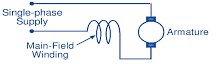
\includegraphics[scale=1.5]{universal/no_compensating_winding.jpg}
    \caption{Circuit diagram of DC motor connected to AC supply}
    \label{fig:no_comp}
\end{figure}


\begin{figure}[h]
    \centering
    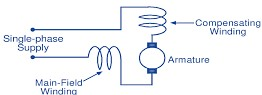
\includegraphics[scale=1.25]{universal/with_compensating_winding.jpg}
    \caption{Circuit diagram of universal motor}
    \label{fig:with_comp}
\end{figure}

To understand the purpose of the compensating winding we must first understand the process that resulted in this design.\\
As previously mentioned, connecting a DC motor to an AC supply results in undesired reactive voltage drop, this voltage drop can be minimized by reducing the number of field turns, reducing the overall flux in the motor. This flux loss is compensated by increasing the number of armature conductors, this can increase the armature reaction, so the compensating winding is added to compensate the effects of the armature reaction. The compensating winding is put in the stator slots. The axis of the compensating winding is 90° (electrical) with the main field axis so the motor's circuit diagram becomes the one shown in figure \ref{fig:with_comp} instead of being the one shown in figure \ref{fig:no_comp}. \cite{guru2007}


\subsection{Advantages Of Universal Motor}
After all the disadvantages mentioned above, and the hurdles that faces whoever attempts to use a universal motor, one might assume that there are no advantages to using a universal motor. But contrary to this belief, there are applications in which a universal motor is desirable such as:
\begin{enumerate}
    \item Applications in which the motor is required to give satisfactory performance when powered by either DC or AC single-phase supply for electric machines used in home. 
    \item Applications that need the motor to automatically adjust its speed according to the load such as saws and sewing machines.
   \item The universal motor is compact and gives more torque per ampere than any other single-phase motor. It is therefore used where light weight and high torque are important. 
    \cite{chapman2005}
\end{enumerate}

\subsection{Speed Control of Universal Motor}
As with dc series motors, the best way to control the speed of a universal motor is 
to vary its rms input voltage. The higher the rms input voltage, the greater the resulting speed of the motor. \cite{chapman2005}



\subsection{Universal Motor vs Single Phase Induction Motor}

\subsubsection{Points regarding universal motor}
\begin{itemize}
    \item Can run on either AC or DC.
    \item High noise ,high speed 4000–16000 rpm, and can go over 20,000 rpm.
    \item Large starting torque.
    \item Carbon brushes  wear out and produce sparks.
    \item Lighter weight since it uses only coils.
    \item  self starting.
\end{itemize}

\subsubsection{Points regarding single phase induction motor}
\begin{itemize}
    \item Runs on AC only.
    \item Induction motors are slow because the rpm depends on the number of poles and the frequency of the supply.
    \item Small starting torque (not even self starting).
    \item No brushes so their parts are built for long life and they run at relatively low speeds.
    \item Large and heavy because the induction process takes a lot of iron and copper.
    \item Not self starting.
\end{itemize}






%%%%%%%%%%%%%%%%%%%%%%%%%%%%%%%%
%%%%%%%%%%%%%%%%%%%%%%%%%%%%%%%%
%%%%%%%%%%%%%%%%%%%%%%%%%%%%%%%%
\section{Stepper Motor}




A stepper motor, also known as step motor or stepping motor, is a brushless DC electric motor that divides a full rotation into a number of equal steps. The motor's position can be commanded to move and hold at one of these steps without any position sensor for feedback (an open-loop controller), as long as the motor is correctly sized to the application in respect to torque and speed.\cite{wikipedia_stepper}


\begin{figure}[!h]
    \centering
    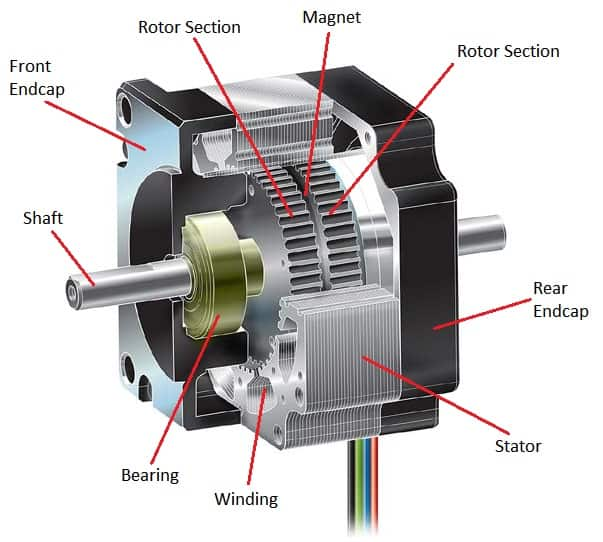
\includegraphics[scale=0.33]{Stepper/stepper1.png}
    \caption{Hybrid Stepper Motor Basic Construction}
    \label{fig:Stepper Construction}
\end{figure}


%\subsection{Explain the theory of stepper motor operation highlighting what makes such machine special.(kero)}
\subsection{Theory of Operation and Construction}

%%%%%%GURU%%%%%%
Step motors (Fig. \ref{fig:Stepper Construction}), also known as stepping or stepper motors, are essentially incremental motion devices. \cite{guru2007}

%%%%%%%%Chapman%%%%%%%%
%\cite{chapman2005}
A stepper motor is a special type of synchronous motor which is designed to rotate a specific number of degrees for every electric pulse received by its control unit. Typical steps are 7.5\textdegree or 15\textdegree per pulse. These motors are used in many control systems, since the position of a shaft or other piece of machinery can be controlled precisely with them. \cite{chapman2005}

A simple stepper motor and its associated control unit are shown in Fig. \ref{fig:Stepper 10-38-a}, Fig. \ref{fig:Stepper 10-38-b}, and Fig. \ref{fig:Stepper 10-38-c}. To understand the operation of the stepper motor, examine Fig. \ref{fig:Stepper 10-39-a}, Fig. \ref{fig:Stepper 10-39-b}, and Fig. \ref{fig:Stepper 10-39-c}. 


This figure shows a two-pole three-phase stator with a permanent-magnet rotor. If a dc voltage is applied to phase a of the stator and no voltage is applied to phases b and c, then a torque will be induced in the rotor which causes it to line up with the stator magnetic field $B_S$, as shown in Fig. \ref{fig:Stepper 10-39-b}.

\begin{figure}[h]
    \centering
    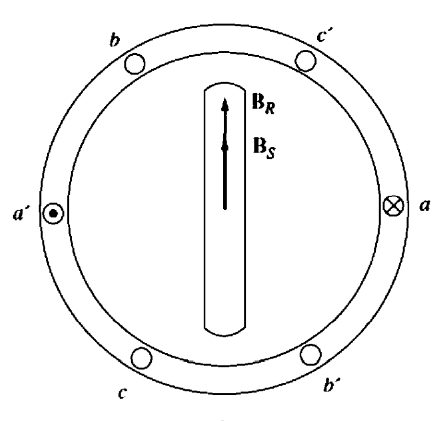
\includegraphics[scale=0.39]{Stepper/fig 10-39-b.PNG}
    \caption{(b) When the rotor lines up with the stator magnetic field. the net torque falls to zero. }
    \label{fig:Stepper 10-39-b}
\end{figure}


\begin{figure}[h]
    \centering
    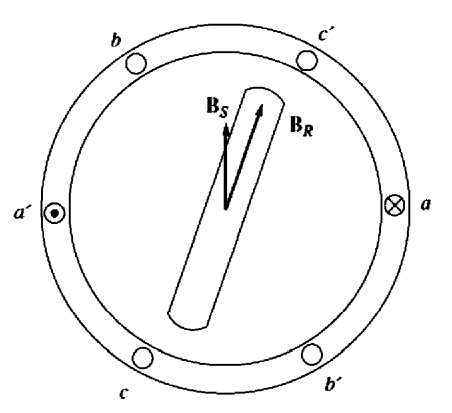
\includegraphics[scale=0.39]{Stepper/fig 10-39-a.PNG}
    \caption{(a) A voltage V is applied to phase a of the stator. causing a current to flow in phase a and producing a stator magnetic field $B_S$. The interaction of $B_R$ and $B_S$ produces a counterclockwise torque on the rotor. }
    \label{fig:Stepper 10-39-a}
\end{figure}

\begin{figure}[h]
    \centering
    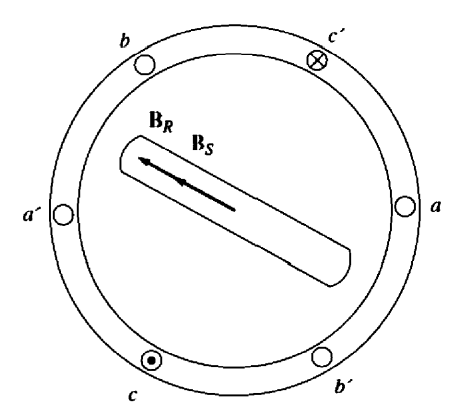
\includegraphics[scale=0.39]{Stepper/fig 10-39-c.PNG}
    \caption{(c) A voltage V is applied to phase c of the stator. causing a current to flow in phase c and producing a stator magnetic field $B_S$. The interaction of $B_R$ and $B_S$ produces a counterclockwise torque on the rotor, causing the rotor to line up with the new position of the magnetic field.}
    \label{fig:Stepper 10-39-c}
\end{figure}







Now assume that phase a is turned off and that a negative dc voltage is applied to phase c. The new stator magnetic field is rotated 60\textdegree with respect to the previous magnetic field, and the rotor of the motor follows it around. By continuing this pattern, it is possible to construct a table showing the rotor position as a function of the voltage applied to the stator of the motor. If the voltage produced by the control unit changes with each input pulse in the order shown in Fig. \ref{fig:Table 10-1}, then the stepper motor will advance by 60\textdegree with each input pulse. 

\begin{figure}[h]
    \centering
    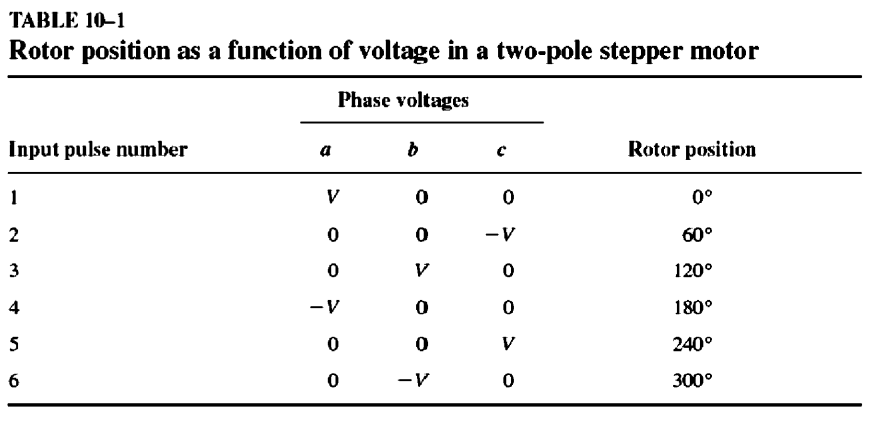
\includegraphics[scale=0.33]{Stepper/table 10-1.PNG}
    \caption{The voltage produced by the control unit changes with each input pulse in the order shown in this table}
    \label{fig:Table 10-1}
\end{figure}

It is easy to build a stepper motor with finer step size by increasing the number of poles on the motor. From $Equation$ \ref{stepper equation 1} the number of mechanical degrees corresponding to a given number of electrical degrees is


\begin{equation}
    \theta_m = \frac{2}{P} \cdot \theta_e
    \label{stepper equation 1}
\end{equation}


Since each step in Table shown in Fig. \ref{fig:Table 10-1} corresponds to 60 electrical degrees, the number of mechanical degrees moved per step decreases with increasing numbers of poles. For example, if the stepper motor has eight poles, then the mechanical angle of the motor's shaft will change by 15\textdegree per step.

The speed of a stepper motor can be related to the number of pulses into its control unit per unit time by using $Equation$ \ref{stepper equation 1}. $Equation$ \ref{stepper equation 1} gives the mechanical angle of a stepper motor as a function of the electrical angle. If both sides of this equation are differentiated with respect to time, then we have a relationship between the electrical and mechanical rotational speeds of the motor: 


\begin{equation}
    \omega_m = \frac{2}{P} \cdot \omega %wm = 2/p*W   ~ (1O-19a) 
\end{equation}

\begin{equation}
    n_m = \frac{2}{P} \cdot n_e  %nm = 2/p*ne   ~ (IO-19b) 
\end{equation}



Since there are six input pulses per electrical revolution, the relationship between the speed of the motor in revolutions per minute and the number of pulses per minute becomes

\begin{equation}
    n_m = \frac{1}{3P} \cdot n_{pulses}
\end{equation}

where $n_{pulses}$ is the number of pulses per minute.

%Figures
%Figures 
%Figures 
%Figures 

\begin{figure}[h]
    \centering
    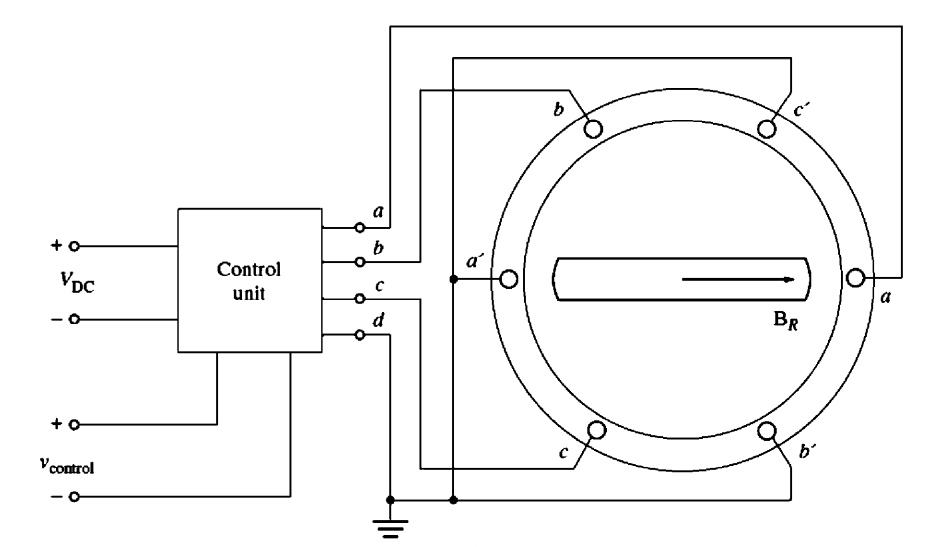
\includegraphics[scale=0.32]{Stepper/fig 10-38-a.PNG}
    \caption{(a) A simple three-phase stepper motor and its associated control unit. The inputs to the control unit consist of a dc power source and a control signal consisting of a train of pulses.}
    \label{fig:Stepper 10-38-a}
\end{figure}

\begin{figure}[h]
    \centering
    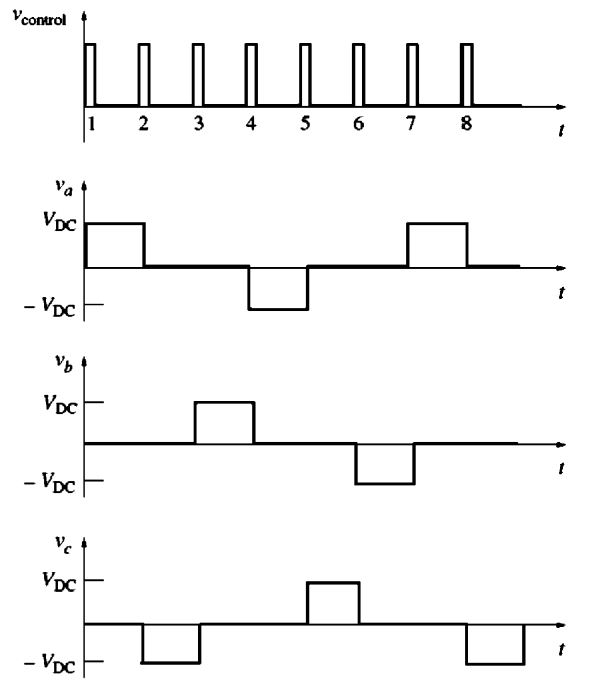
\includegraphics[scale=0.32]{Stepper/fig 10-38-b.PNG}
    \caption{(b) A sketch of the output voltage from the control unit as a series of control pulses are input. }
    \label{fig:Stepper 10-38-b}
\end{figure}

\begin{figure}[h]
    \centering
    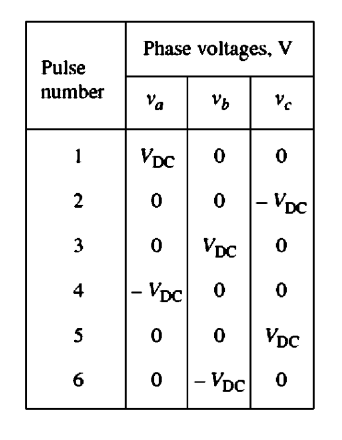
\includegraphics[scale=0.45]{Stepper/fig 10-38-c.PNG}
    \caption{(c) A table showing the output voltage from the control unit as a function of pulse number.}
    \label{fig:Stepper 10-38-c}
\end{figure}


%\subsection{Explain why stepper motors are being utilized.(both)}
\subsection{Utilization of Stepper Motors}


%%applications
A step motor receives a rectangular pulse train and responds by rotating its shaft a certain number of degrees as dictated by the number of pulses in the pulse train. Usually the pulse train is controlled by means of a microcomputer or an electronic circuit. As a result, a step motor is very much compatible with digital electronic circuits and may form an interface between a microcomputer and a mechanical system. 
Since the motion in a step motor is generally governed by counting the number of pulses, no feedback loops and sensors are needed for its control. Therefore, step motors are suitable for position control in an open loop system. They are relatively inexpensive and simple in construction and can be made to step in equal increments in either direction. \cite{guru2007}

Step motors are excellent candidates for such applications as printers, XY plotters, electric typewriters, control of floppy disk drives, robots, and numerical control of machine tools. \cite{guru2007}


In the field of lasers and optics they are frequently used in precision positioning equipment such as linear actuators, linear stages, rotation stages, goniometers, and mirror mounts. Other uses are in packaging machinery, and positioning of valve pilot stages for fluid control systems.\cite{wikipedia_stepper}

Commercially, stepper motors are used in floppy disk drives, flatbed scanners, computer printers, plotters, slot machines, image scanners, compact disc drives, intelligent lighting, camera lenses, CNC machines, and 3D printers.\cite{wikipedia_stepper}



%\subsection{What are the different types of stepper motors, mentioning construction and properties of each type.(Sherif)} 
\subsection{Different Types and Their Construction}

Stepper motors are classified according to \textbf{the structure of rotor} into one of three categories:\textbf{Variable Reluctance Stepper Motor, Permanent Magnet Rotor Stepper Motor}, and \textbf{Hybrid Stepper Motor}. \cite{rizzoni2007}\cite{stepperNotes} 

\subsubsection{Variable Reluctance Stepper Motor}\hfill\\
As shown in figure \ref{vrS}, a variable reluctance (VR) stepper motor consists of a a soft iron multi-toothed rotor and a laminated wound stator. The rotor does not carry any windings. Therefore, to make one set of rotor and stator poles align,  the number of teeth in the rotor are made different from the stator. \cite{guru2007} \cite{rizzoni2007} \\
\begin{figure}[h]
    \centering
    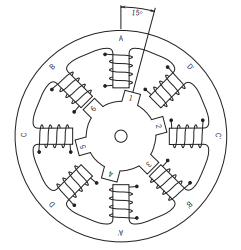
\includegraphics[scale=0.78]{Stepper/vrStep.png}
    \caption{Cross-Section of a VR Stepper Motor}
    \label{vrS}
\end{figure}

\textbf{Properties:}\cite{chapman2005} \cite{rizzoni2007}. \\
\begin{enumerate}
    \item The rotor inertia is low, so the response is very quick. However, it has a low allowable load inertia.
    \item The static torque affecting the rotor equals zero; meaning that no torque affects the rotor when the motor is not energized.
    \item Generally, the step angle of a VR stepper motor is 15$^{\circ}$.
    \item The torque in a reluctance motor is directly proportional to $sin 2{\delta}$, where ${\delta}$ is the step angle. Therefore, stepper motors are bulit with four-phase stator winding (as shown in figure \ref{vrS}) instead of three, producing a higher torque on the rotor.
\end{enumerate}



\subsubsection{Permanent Magnet Rotor Stepper Motor}\hfill\\
It is a low cost, and low precision stepper motor.   
Unlike the rotor of a VR stepper motor, the rotor of a PM (also referred as "tin-can") stepper motor does not have teeth. Instead, it consists of permanent magnets, with alternating north and south poles situated in a straight line parallel to the rotor shaft (As in figure \ref{pmS}). The stator of PM stepper motor is the same as its VR counterpart. \cite{guru2007} \cite{stepperNotes} \\

\begin{figure}[h]
    \centering
    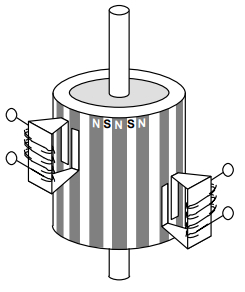
\includegraphics[scale=0.7]{Stepper/pmStep.png}
    \caption{Cross-Section of a PM Stepper Motor}
    \label{pmS}
\end{figure}



\textbf{Properties:}\cite{chapman2005} \cite{stepperNotes}. \\
\begin{enumerate}
    \item The sturcture of the rotor provides the PM stepper motor with improved torque characteristics compared with the VR type.
    \item The step angle of a PM stepper can be 7.5$^{\circ}$, 11.25$^{\circ}$, 15$^{\circ}$, 18$^{\circ}$, 45$^{\circ}$, or 90$^{\circ}$, depending on the number of stator poles.
    
\end{enumerate}




\subsubsection{Hybrid Stepper Motor}\hfill\\
%%%%%%%%%%%%%%%%%%%%%%%%%%%%%%%%%%%%%%%%%
The Hybrid (HB) Stepper motor is one of most used stepper motors, beside the PM type. However, it is more expensive, providing s better performance with respect to step resolution, torque and speed. While the stator is no different from that of a VR or PM stepper motors, its rotor combines the main features of the aforementioned motor types. The rotor, as seen in figure \ref{hbS}consists of two identical stacks of multi-toothed soft iron (like the VR stepper), as well as axially magnetized round permanent magnet (similar to PM stepper). \\The soft iron stacks are attached to the poles of the magnet, magnetizing one side of rotor teeth to north pole, and the other to south pole. The rotor teeth at both north and south poles are displaced in angle for the proper alignment of the rotor pole with that of the stator. \cite{guru2007} \cite{stepperNotes} 
\begin{figure}[h]
    \centering
    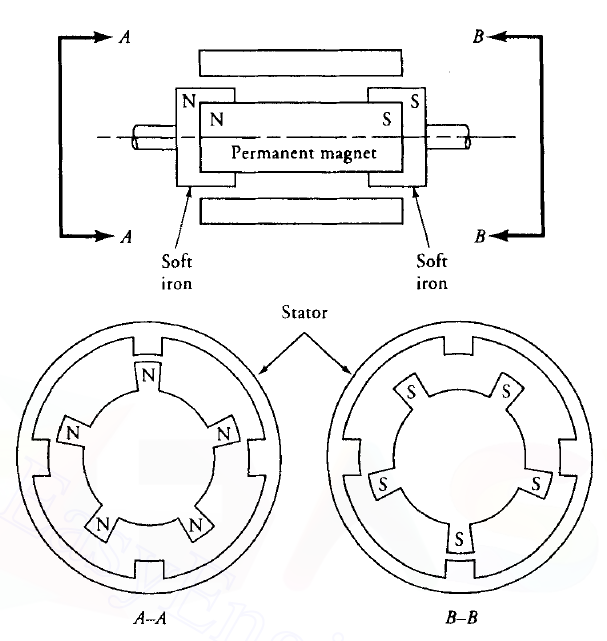
\includegraphics[scale=0.5]{Stepper/hbStep.png}
    \caption{Various views of a hybrid stepper motor.}
    \label{hbS}
\end{figure}


\textbf{Properties:}\cite{rizzoni2007} \cite{stepperNotes}. \\
\begin{enumerate}
    \item The use of both permanent magnets and high permeability iron core in the stator provides the motor with higher torque than its counterparts.
    \item IT has high accuracy. Typical step angles for the HB stepper motor range from 3.6\textdegree to 0.9\textdegree.
    
\end{enumerate}
%%%%%%%%%%%%%

\textbf{How the teeth are arranged:}

\begin{figure}[h]
    \centering
    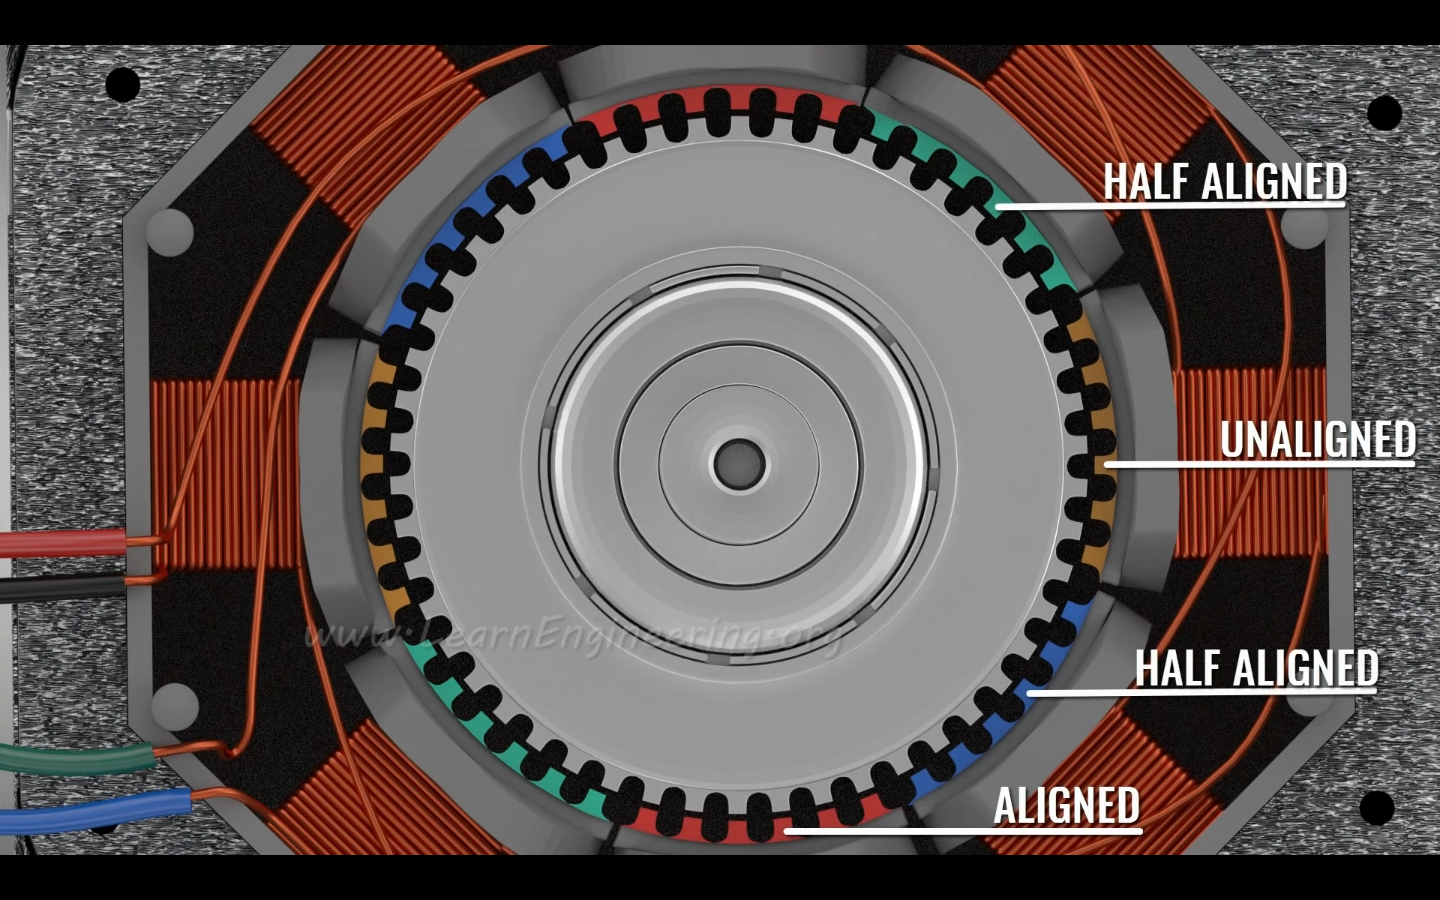
\includegraphics[trim={0 2cm 0 2cm} ,clip,scale=0.15]{Stepper/stepper teeth hybrid.png}
    \caption{\centering The Teeth of the hybrid 1.8\textdegree step size Hybrid Stepper Motor.}
    \label{teeth hybrid}
\end{figure}

The accuracy of this motor type lies in the clever arrangement of the rotor and stator teeth. In this 1.8\textdegree step motor, the rotor has 50 teeth. The stator has two fewer teeth than the rotor, that is 48 teeth. Let us arrange the 48 teeth into 4 group coloured as shown in figure \ref{teeth hybrid}. The red set is completely aligned with the teeth of the rotor. The yellow set is unaligned. The blue and green are half-aligned. Let the rotor that is facing upwards is the south pole. The north end cap teeth is unaligned with the south end cap teeth, in other words, the north end cap teeth are placed in between the south end cap teeth. When coils set A is energized, the stator forms a magnetizing pattern so the same polarity poles will be unaligned, the opposite poles will align as they attract. When B is energized, the rotor will move a small angle so that the south poles align with the new north poles.
This step can be calculated by this equation: 

\begin{equation} \label{eq1}
\begin{split}
Step Angle & =  \frac{1}{4} \cdot Angular Pitch \\
 & = \frac{1}{4} \cdot 7.2 = 1.8
\end{split}
\end{equation}

The Angular Pitch can be calculated by: 
\begin{equation}
    Angular Pitch = \frac{360}{50} = 7.2
\end{equation}
, where 50 is the number of the rotor teeth.


Again, set A is energized with opposite polarity and so on. We get a very high accurate step motion from the motor. step angle resolution can be further improved by half stepping. 



%\subsection{With proper schematic, explain the winding types of stepper motor mentioning how it operates with each type.(Sherif)} 
\subsection{Different Types: Winding, Schematic and Operation}
Previously, stepper motors were characterized according to the construction of rotor. However, stepper motors can be classified according to the type of stator winding into: \textbf{Variable Reluctance Stepper Motor, Unipolar Stepper Motor, Biploar Stepper Motor}, and \textbf{Bifilar Stepper Motor}. \cite{stepTypes_stepper}\\

\subsubsection{Variable Reluctance Stepper Motor}\hfill\\
In a VR stepper motor, the windings are usually connected at one terminal, usually going to the positive supply, and the windings are energized in sequence.\\
\begin{figure}[h]
    \centering
    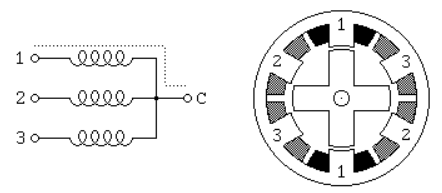
\includegraphics[scale=0.63]{Stepper/vrStep2.png}
    \caption{The windings of a VR stepper motor}
    \label{vrS2}
\end{figure}
In figure \ref{vrS2}, a cross-section of a VR stepper, with 4 rotor teeth, 6 stator poles, 30\textdegree per step, and each winding wrapped around two opposite poles. When winding 1 is energized, the rotor upper and lower teeth are attracted to the poles with that winding. If winding 1 is turned off and winding 2 is turned on, the rotor rotates 30\textdegree clockwise; as its left and right poles are attracted to the poles of winding 2.\\For the rotor to continue rotating clockwise, power is applied to the 3 windings in sequence.  Table \ref{vrCTRL} shows the control sequence for the VR stepper, spinning the motor 8 steps clockwise, assuming \textbf{"H"} means turning on the current through motor winding.

\begin{table}[h!]
\begin{center}
\begin{tabularx}{0.47\textwidth} { 
  | >{\raggedleft\arraybackslash}X 
  | >{\centering\arraybackslash}X 
  | >{\centering\arraybackslash}X 
  | >{\centering\arraybackslash}X
  | >{\centering\arraybackslash}X
  | >{\centering\arraybackslash}X
  | >{\centering\arraybackslash}X
  | >{\centering\arraybackslash}X
  | >{\centering\arraybackslash}X
  | >{\centering\arraybackslash}X
  | >{\centering\arraybackslash}X|}
 \hline
  Coil & \multicolumn{3}{|c|}{Cycle 1} & \multicolumn{3}{|c|}{Cycle 2} & \multicolumn{3}{|c|}{Cycle 3} \\
 \hline  
 W1 & H & L & L & H & L & L & H & L & L \\
 \hline
 W2 & L & H & L & L & H & L & L & H & L \\
\hline
 W3 & L & L & H & L & L & H & L & L & H\\
 \hline
\end{tabularx}
 \caption{Control Sequence of VR Stepper Motor. (One phase on-Full step)}
\label{vrCTRL}
\end{center}
\end{table}

\subsubsection{Unipolar Stepper Motor}\hfill\\
Usually, this winding method is found in both PM and HB stepping motors, with a center tap on each of two windings. The center tap is typically wired to the positive supply, while the two ends are alternately grounded to reverse the direction of the field provided by that winding.\\

\begin{figure}[h]
    \centering
    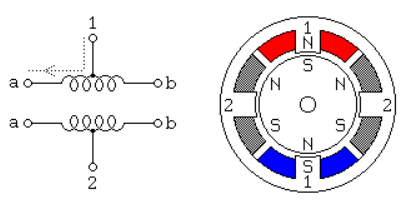
\includegraphics[scale=0.63]{Stepper/uPStep.png}
    \caption{The windings of a unipolar stepper motor}
    \label{upS}
\end{figure}
Figure \ref{upS} shows a 4-pole stator, 6-pole rotor permanent magnet or hybrid stepper motor with 30\textdegree per step. Winding 1 is distributed between top and bottom stator poles, and winding 2 is distributed between the left and right poles. When current flows from the center tap of winding 1 to terminal \textbf{a}, the top stator pole becomes the north pole while the bottom pole becomes the south pole, attracting the rotor into the position shown in figure \ref{upS}.\\
When winding \textbf{1a} is denergized, and winding \textbf{2a} is turned on, the rotor will turn 30\textdegree clockwise or one step.\\

To rotate the unipolar stepper motor continuously, power is applied to the two windings in sequence.  Tables \ref{upCTRL1} and \ref{upCTRL2} show the control sequence for the unipolar stepper, spinning the motor 9 steps clockwise, assuming \textbf{"H"} means turning on the current through motor winding.


\begin{table}[h!]
\begin{center}
\begin{tabularx}{0.47\textwidth} { 
  | >{\raggedright\arraybackslash}X 
  | >{\centering\arraybackslash}X 
  | >{\centering\arraybackslash}X 
  | >{\centering\arraybackslash}X
  | >{\centering\arraybackslash}X
  | >{\centering\arraybackslash}X
  | >{\centering\arraybackslash}X
  | >{\centering\arraybackslash}X
  | >{\centering\arraybackslash}X
  | >{\centering\arraybackslash}X
  | >{\centering\arraybackslash}X|}
 \hline
 Coil & \multicolumn{4}{|c|}{Cycle 1} & \multicolumn{4}{|c|}{Cycle 2} & \multicolumn{2}{|c|}{Cycle 3} \\
 \hline  
 1a & H & L & L & L & H & L & L & L & H & L\\
 \hline
 1b & L & L & H & L & L & L & H & L & L & L\\
\hline
 2a & L & H & L & L & L & H & L & L & L & H\\
 \hline
 2b & L & L & L & H & L & L & L & H & L & L\\
 \hline
\end{tabularx}
 \caption{Control Sequence of unipolar Stepper Motor (One phase on-Full step).}
\label{upCTRL1}
\end{center}
\end{table}

\begin{table}[h!]
\begin{center}
\begin{tabularx}{0.47\textwidth} { 
  | >{\raggedright\arraybackslash}X 
  | >{\centering\arraybackslash}X 
  | >{\centering\arraybackslash}X 
  | >{\centering\arraybackslash}X
  | >{\centering\arraybackslash}X
  | >{\centering\arraybackslash}X
  | >{\centering\arraybackslash}X
  | >{\centering\arraybackslash}X
  | >{\centering\arraybackslash}X
  | >{\centering\arraybackslash}X
  | >{\centering\arraybackslash}X|}
 \hline
 Coil & \multicolumn{4}{|c|}{Cycle 1} & \multicolumn{4}{|c|}{Cycle 2} & \multicolumn{2}{|c|}{Cycle 3} \\
 \hline  
 1a & H & H & L & L & H & H & L & L & H & H\\
 \hline
 1b & L & L & H & H & L & L & H & H & L & L\\
\hline
 2a & L & H & H & L & L & H & H & L & L & H\\
 \hline
 2b & H & L & L & H & H & L & L & H & H & L\\
 \hline
\end{tabularx}
 \caption{Control Sequence of unipolar Stepper Motor (Two phases on-Full step).}
\label{upCTRL2}
\end{center}
\end{table}

\textbf{Regarding The Unipolar stepper motor:} \\
\begin{enumerate}
    \item The two halves of each winding are never energized at the same time.
    \item The aforementioned sequences in tables \ref{upCTRL1}, \ref{upCTRL2} will rotate the unipolar PM or HB stepper motor one step at a time. \textbf{The first sequence} uses less power, while \textbf{the second sequence} uses twice as much power, producing about 1.4 times greater torque.
\end{enumerate}

\subsubsection{Bipolar Stepper Motor}\hfill\\
Bipolar PM and HB stepper motors are constructed with exactly the same mechanism that is used on unipolar motors. The only exception is that two windings are wired with no center taps for simpler winding. Despite the simpler motor, the required drive circuitry becomes more complex; as it has to be able to reverse the polarity of each pair of motor poles. Such task can be accomplished by using \textbf{H-Bridge Control Circuit} for each winding.\\

\begin{figure}[h]
    \centering
    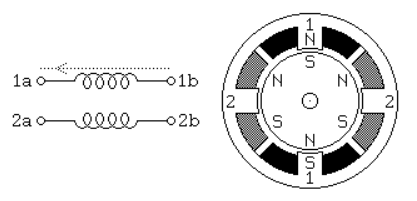
\includegraphics[scale=0.64]{Stepper/bPStep.png}
    \caption{The windings of a bipolar stepper motor.}
    \label{bpS}
\end{figure}
The driving sequence of a bipolar motor is identical to that for a unipolar motor at an abstract level. The main difference is that polarity of each winding is reversed every time it is energized.\\

\begin{table}[h!]
\begin{center}
\begin{tabularx}{0.47\textwidth} { 
  | >{\raggedright\arraybackslash}X 
  | >{\centering\arraybackslash}X 
  | >{\centering\arraybackslash}X 
  | >{\centering\arraybackslash}X
  | >{\centering\arraybackslash}X
  | >{\centering\arraybackslash}X
  | >{\centering\arraybackslash}X
  | >{\centering\arraybackslash}X
  | >{\centering\arraybackslash}X
  | >{\centering\arraybackslash}X
  | >{\centering\arraybackslash}X|}
 \hline
 Coil & \multicolumn{4}{|c|}{Cycle 1} & \multicolumn{4}{|c|}{Cycle 2} & \multicolumn{2}{|c|}{Cycle 3} \\
 \hline  
 1a & + & - & - & - & + & - & - & - & + & -\\
 \hline
 1b & - & - & + & - & - & - & + & - & - & -\\
\hline
 2a & - & + & - & - & - & + & - & - & - & +\\
 \hline
 2b & - & - & - & + & - & - & - & + & - & -\\
 \hline
\end{tabularx}
 \caption{Control Sequence of bipolar Stepper Motor (One phase on-Full step).}
\label{bpCTRL1}
\end{center}
\end{table}

\begin{table}[h!]
\begin{center}
\begin{tabularx}{0.47\textwidth} { 
  | >{\raggedright\arraybackslash}X 
  | >{\centering\arraybackslash}X 
  | >{\centering\arraybackslash}X 
  | >{\centering\arraybackslash}X
  | >{\centering\arraybackslash}X
  | >{\centering\arraybackslash}X
  | >{\centering\arraybackslash}X
  | >{\centering\arraybackslash}X
  | >{\centering\arraybackslash}X
  | >{\centering\arraybackslash}X
  | >{\centering\arraybackslash}X|}
 \hline
 Coil & \multicolumn{4}{|c|}{Cycle 1} & \multicolumn{4}{|c|}{Cycle 2} & \multicolumn{2}{|c|}{Cycle 3} \\
 \hline  
 1a & + & + & - & - & + & + & - & - & + & +\\
 \hline
 1b & - & - & + & + & - & - & + & + & - & -\\
\hline
 2a & - & + & + & - & - & + & + & - & - & +\\
 \hline
 2b & + & - & - & + & + & - & - & + & + & -\\
 \hline
\end{tabularx}
 \caption{Control Sequence of bipolar Stepper Motor (Two phases on-Full step).}
\label{upCTRL2}
\end{center}
\end{table}

\textbf{Regarding The Bipolar stepper motor:}\\
We can distinguish between a bipolar permanent magnet motor from other 4 wire motors by measuring the resistance between different terminals.  Some permanent magnet stepping motors have 4 independent windings, organized as two sets of two. Within each set:
\begin{itemize}
    \item  If the two windings are wired in series, the result can be used as a high voltage bipolar motor.
    \item If they are wired in parallel, the result can be used as a low voltage bipolar motor.
    \item If they are wired in series with a center tap, the result can be used as a low voltage unipolar motor.
\end{itemize}

\subsubsection{Bifilar Motors}\hfill

Using the same rotor and stator geometry as a bipolar motor, bifilar windings can be applied on that stepper motor. The only difference is that each coil in the stator is wound using two wires in parallel with each other, resulting in a motor with 8 wires.\\

\begin{figure}[h]
    \centering
    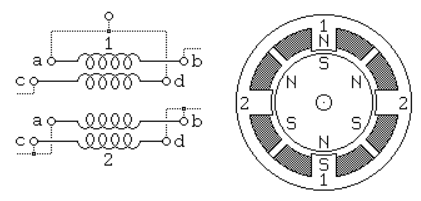
\includegraphics[scale=0.75]{Stepper/bifiliarStep.png}
    \caption{Bifilar windings on a stepper motor.}
    \label{bifilar}
\end{figure}
Practically, motors with bifilar windings can be powered as either unipolar or bipolar motors. To use stepper motor as:
\begin{itemize}
    \item \textbf{Unipolar Motor:} The two wires of each winding are connected in  series, and the point of connection is used as a center-tap. (As showm in figure \ref{bifilar})
    \item \textbf{Bipolar Motor:} The two wires of each winding are connected in parallel (for low-voltage high-current operation) or in series, ignoring the center-tap (for low-current high-voltage operation).
\end{itemize}
Naturally, unipolar motors may be used as bipolar motors at twice the voltage rating and half the current rating.\\
To ensure correct operation of the a bifilar motor, three issues are taken into consideration: The current carrying capacity of the wire, cooling the motor, and avoiding driving the motor's magnetic circuits into saturation.\\


%%%%%%%%%%%%%
\subsection{Speed-torque characteristic of a step motor:}
\begin{figure}[h]
    \centering
    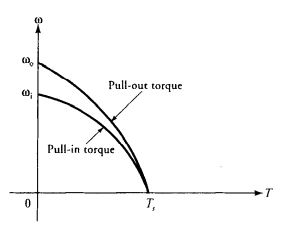
\includegraphics[scale=0.7]{Stepper/speed-torque characteristic for step motor.PNG}
    \caption{Speed-torque characteristic of a step motor.}
    \label{speed torque graph}
\end{figure}


Step motors are generally used in a range from 1 Watt to about 3 hp, and their step sizes vary from approximately 0.72\textdegree to 90\textdegree. However, the most common step sizes are 1.8\textdegree, 7.5\textdegree, and 15\textdegree. 
Since a step motor rotates when a series of pulses is applied to its phase windings, the duration of each pulse should be sufficiently long to accurately rotate the motor at the desired speed. If the pulse duration is too short, the rotor will miss the steps and be unable to follow the applied pulses accurately. Thus either the motor will not rotate or the required speed will not be achieved. To avoid such an undesirable operation, usually the pulse duration is selected so that it is greater than the inertial time-constant of the combination of the rotor and the mechanical load. Therefore, it is expected that a large motor with a high moment of inertia requires a slower pulse rate for accurate operation. 

The pull-in torque characteristic shown in Figure \ref{speed torque graph} illustrates the permissible range of rate of steps for a given load and a motor in order not to miss a step. When the motor achieves its steady-state operation, the speed is uniform and no starting and stopping take place at each step. We can load the motor up to a limit, which is defined by the pull-out torque characteristic shown in Figure \ref{speed torque graph}. Above that torque level the motor starts missing the steps, thereby losing speed. \cite{guru2007}







%\subsection{A single-stack stepper motor producing 200 steps/rev, it’s desired to obtain half-step angle, explain how to realize this desired angle with two different driving methods. Explaining the advantages and disadvantages of each method.(practical: like a question in exam)}
\subsection{Half-Stepping and Micro-Stepping:}


Let there be a single-stack stepper motor producing 200 steps/rev, it’s desired to obtain half-step angle, that will make it produce 400 steps/rev. A way to realize this desired angle with two different driving methods will be given. Explaining the advantages and disadvantages of each method.


There are two types of full step excitation modes.
In one-phase on - full step, the motor is operated with only one phase energized at a time. This mode requires the least amount of power from the driver of any of the excitation modes.

In two-phase on - full step, the motor is operated with both phases energized at the same time. This mode provides improved torque and speed performance. Two-phase on provides about 30\% to 40\% more torque than one phase on, however it requires twice as much power from the driver.

Half step excitation mode is a combination of one phase on and two phase on full step modes. This results in half the basic step angle. This smaller step angle provides smoother operation due the increased resolution of the angle.

Half step produces about 15\% less torque than two phase on - full step, however modified half stepping eliminates the torque decrease by increasing the current applied to the motor when a single phase is energized. See Fig. \ref{half stepping}. \cite{website_microstep}


\begin{figure}[h]
    \centering
    % trim from bottom edge
    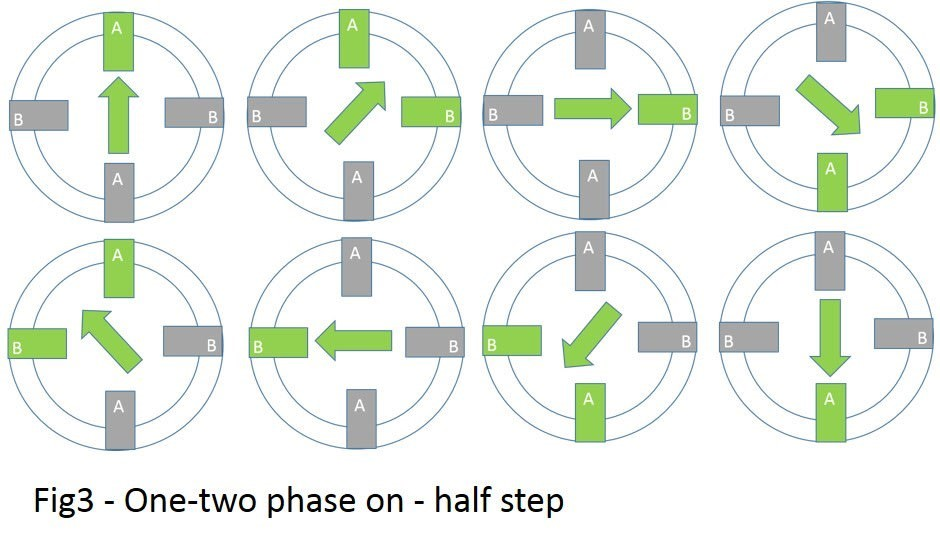
\includegraphics[trim={0 2cm 0 0},clip,scale=0.34]{Stepper/halfstep.jpg}
    \caption{A single-stack stepper motor. Half- stepping.}
    \label{half stepping}
\end{figure}



%kero's speculation
%for half stepping two adjacent coils shall be energized at the same time. the coil will position itself half way between them. hence, half step. this is method one.
%method two.. idk .. i think it has to do with micro stepping

%The second method has to do with the motor driver or the micro-controller responsible for adjusting the energizing voltage and current into the stepper motor coils.

This was the first driving way. The second way is by Microstepping, another form of getting more steps from the stepper motor.
%%%todo: the second way is still unknown
Microstepping can divide a motor’s basic step by up to 256 times, making small steps smaller. A Micro drive uses two current sinewaves 90\textdegree apart, this is perfect for enabling smooth running of the motor. You will notice that the motor runs is quietly and with no real detectable stepping action.

By controlling direction and amplitude of the current flow in each winding, the resolution increases and the characteristics of the motor improve, giving less vibration and smoother operation. Because the sinewaves work together there is a smooth transition from one winding to the other. When current increases in one it decreases in the other resulting in a smooth step progression and maintained torque output.\cite{website_microstep}


There are some problems associated with microstepping, mostly accuracy and torque. Because the phases are only phases are only partially energized, the motor torque is reduced, usually by about 30\%. Also because the torque differential between steps is so small, the motor sometimes cannot overcome the load. In those cases the motor may be commanded to move 10 steps before it actually starts to move. In many cases it is necessary to close the loop with encoders (Type of position sensors) which add to the price.\cite{microstep_last_website}





%\subsection{Enumerate the advantages and disadvantages of stepper motor.(kero)}
\subsection{Stepper Motor: The advantages and disadvantages}

The stepper Motor harness a lot of advantages that give it the fame it collected. The advantages can be summarized in a list here:
\begin{enumerate}
    
    \item Low cost for control achieved, High torque at startup and low speeds, Ruggedness, Simplicity of construction, Can operate in an open loop control system, High reliability
    \item Low maintenance, Less likely to stall or slip, Will work in any environment, Can be used in robotics in a wide scale.
    \item The rotation angle of the motor is proportional to the input pulse.
    \item The motor has full torque at standstill (if the windings are energized)
    \item Precise positioning and repeatability of movement since good stepper motors have an accuracy of 3–5\% of a step and this error is non-cumulative from one step to the next.
    \item Excellent response to starting/stopping/reversing.
    \item Very reliable since there are no contact brushes in the motor. Therefore, the life of the motor is simply dependent on the life of the bearing.
    \item The motors response to digital input pulses provides open-loop control, making the motor simpler and less costly to control.
    \item It is possible to achieve very low-speed synchronous rotation with a load that is directly coupled to the shaft.
    \item A wide range of rotational speeds can be realized as the speed is proportional to the frequency of the input pulses.\cite{wikipedia_stepper}

\end{enumerate}


Some of the drawbacks of step motors can be summarized in a list here:
\begin{enumerate}
    \item The efficiency of the stepper motor is low.
    \item Resonance is the main problem that occurs in variable reluctance motors.\cite{website2_stepper} Their step response may be oscillatory in nature with a considerable overshoot.\cite{guru2007}
    %\item The feedback loop is not used.
    \item They do not offer the flexibility of adjusting the angle of advance. \cite{guru2007}
    \item These motors produce extremely high noise. Not easy to operate extremely at high speeds.
    \item Stepper-motors cannot run or rotate at high speeds but have a high holding torque\cite{website2_stepper}
\end{enumerate}



%\newpage
\bibliographystyle{IEEEtran}
\bibliography{references}	




\end{document}
